%--------------------
% Packages
% -------------------
\documentclass[11.5pt,a4paper]{article}

\usepackage{indentfirst}
\usepackage[utf8x]{inputenc}
\usepackage[T1]{fontenc}
%\usepackage{gentium}
\usepackage{mathptmx} % Use Times Font
\usepackage{mathtools,amssymb,amsthm}
\usepackage{caption}
\usepackage{tabularx}
\usepackage{mathrsfs}
\usepackage{hyperref}
%\def\Laplace#1{\mathscr{L}_{\scriptscriptstyle\mathscr{O}\mathscr{V}\mathscr{E}}\{#1\}}

\usepackage{siunitx}

\usepackage[pdftex]{graphicx} % Required for including pictures
\usepackage{calc} % To reset the counter in the document after the title page
\usepackage{enumitem} % Includes lists

\usepackage[a4paper, left=1in, right=1in, top=1in, bottom=1in]{geometry} %margins

\usepackage[all]{nowidow} % Tries to remove widows
\usepackage[protrusion=true,expansion=true]{microtype} % Improves typography, lhttps://www.overleaf.com/project/65464d4a52b0d7a8ee25fd6coad after fontpackage is selected

\usepackage{lipsum} % Used for inserting dummy 'Lorem ipsum' text into the template

% Using \doublespacing in the preamble 
% changes the text to double-line spacing
\usepackage{setspace}
\onehalfspacing

\usepackage{color} % for the command \textcolor
\usepackage{soul} % for the command \hl


\usepackage[font=small,labelfont=bf, figurename=Fig.]{caption} 
\renewcommand{\figurename}{Figure}

\newenvironment{conditions}
  {\par\vspace{\abovedisplayskip}\noindent\begin{tabular}{>{$}l<{$} @{${}={}$} l}}
  {\end{tabular}\par\vspace{\belowdisplayskip}}

\usepackage{verbatim}

%-----------------------
% Begin document
%-----------------------
\begin{document} 

\noindent  Bhargav Akula Ramesh Kumar\\
\textbf{Date: } Nov 16, 2024\\
\begin{center}
    \textbf{Notes on Data-Drive Science and Engineering}
\end{center}

\section{Singular Value Decomposition (SVD)}

\begin{itemize}
    \item Definition SVD: Computational-based method of extracting patterns from high-dimensional data sets
    \begin{itemize}
        \item This is done by extracting "low rank" (number of linearly independent columns or dimension of the column space) approximations for a matrix and performing an inverse/pseudo-inverse to determine a solution to a system of equations in the form $Ax = b$
        \item **\textbf{Low-rank approximations of a matrix}** refer to techniques used to approximate a given matrix \( A \) by another matrix \( \tilde{A} \) that has a lower rank than \( A \).
        \item \href{https://www.youtube.com/watch?v=CpD9XlTu3ys}{What is SVD - Youtube Video}
    \end{itemize}
    \item In other words, it provides a low-dimensional approximation of high-dimensional data through dominant patterns (DATA-DRIVEN APPROACH!)
\end{itemize}

\subsection*{Overview}

\begin{itemize}
    \item General Equation for SVD: $X = U\Sigma V^{*}$. The SVD is a transformation of the orthonormal basis \( \{ \mathbf{v}_i \} \) of the input space into the output space, resulting in the scaled orthonormal basis \( \{ \sigma_i \mathbf{u}_i \} \).
 Below is the derivation:
    \begin{align*}
        AV &= U\sum \\
        A &= U\sum V^*
    \end{align*}
    \begin{itemize}
        \item for $X \in \mathbb{C}^{n,m}$, $U \in \mathbb{C}^{n,n}$ and $V \in \mathbb{C}^{m,m}$
        \begin{itemize}
            \item \textbf{From ChatGPT:} $U$ represent the left singular vectors (the output space that $X$ acts onto) while $V$ represents the right singular vectors (the input space that $X$ acts on). 
            \item The singular vectors show the variability and information captured by the corresponding singular vectors. In other words, the larger the singular value, the greater impact that a small change in the input singular vector (right singular vector) will have on the output singular vector (left singular vector)
        \end{itemize}
        \item \textit{the "*" represents CONJUGATE TRANSPOSE}
        \begin{itemize}
            \item \textit{The conjugate transpose is derived by first taking the transpose of the matrix and then determining the complex conjugate for each value in the matrix. For matrices in the real space, the conjugate transpose is the same as the transpose of the matrix.}
        \end{itemize}
        \item the eigendecomposition of $A^TA$ allows one to determine $V$
        \item the eigendecomposition of $AA^T$ allows one to determine $U$
        \item if $X$ doesn't have full rank, one can use the \textbf{economy SVD}:
        \begin{equation*}
            X = U\sum V^* = \begin{bmatrix} \hat U & \hat U^\perp\end{bmatrix}\begin{bmatrix} \hat \sum \\ 0 \end{bmatrix}V^*
        \end{equation*}
        Where columns of $\hat U^\perp$ spans a vector space that is complementary and orthogonal to $\hat U$. In the economy SVD, this complementary vector ($\hat U^\perp$) it is associated with singular values equal to 0. As a result, the following equation is derived:
        \begin{equation*}
            X = \hat U\hat \sum V^*
        \end{equation*}
        \textit{The above equation is under the assumption that $n \geq m$ for $X \in \mathbb{C}^{n\time m}$}
    \end{itemize}
    \item How does one numerically compute the SVD?
    \begin{itemize}
        \item Can be determined by reducing the matrix $X$ into a bi-diagonal matrix and then iteratively computing the SVD of the bidiagonal matrix
        \item Another method involves using the QR factorization and getting the upper triangular matrix and using the "Householder transformation" to convert it into a bidiagonal matrix.
        \begin{itemize}
            \item QR factorization (or QR decomposition) is a method in linear algebra for decomposing a matrix into a product of two matrices: an orthogonal matrix \( Q \) and an upper triangular matrix \( R \). Specifically, for a given matrix \( A \) (which can be \( m \times n \), with \( m \geq n \)), QR factorization expresses \( A \) as: \[ A = Q R \] Where: 
            \begin{itemize}
                \item \( Q \) is an orthogonal matrix, meaning that its columns are orthonormal vectors (\( Q^T Q = I \), where \( I \) is the identity matrix).

                \textit{\textbf{Note:} In the context of matrices, orthogonal and orthonormal are often used interchangeably when referring to the columns (or rows) of a matrix, especially in real space. This is because, for a square matrix, if its columns (or rows) are orthogonal, they are often assumed to be of unit length as well, making them orthonormal.}\newline
                \item \( R \) is an upper triangular matrix, where all elements below the diagonal are zero.
            \end{itemize}
            QR factorization is useful in various applications such as solving linear systems, least squares problems, and eigenvalue problems. The QR factorization can be found using Gram-Schmidt, Householder transformations, or Givens rotations.
        \end{itemize}
        \item What is a Bidiagonal Matrix?
        \begin{itemize}
            \item A **bidiagonal matrix** is a type of square matrix that has non-zero elements only on the main diagonal and either the superdiagonal (the diagonal just above the main diagonal) or the subdiagonal (the diagonal just below the main diagonal). In other words, a bidiagonal matrix has the following structure:
            \begin{enumerate}
                \item The elements on the main diagonal can be any values.
                \item The elements directly above or below the main diagonal (depending on whether it is an upper or lower bidiagonal matrix) can also be non-zero, but all other elements are zero.
            \end{enumerate}

            \item There are two types of bidiagonal matrices:
            \begin{enumerate}
                \item **Upper bidiagonal matrix**: Non-zero elements appear on the main diagonal and the super-diagonal (above the main diagonal), while all other elements are zero.
               \[
               B = \begin{bmatrix}
               b_{11} & b_{12} & 0 & 0 & \cdots & 0 \\
               0 & b_{22} & b_{23} & 0 & \cdots & 0 \\
               0 & 0 & b_{33} & b_{34} & \cdots & 0 \\
               \vdots & \vdots & \vdots & \vdots & \ddots & \vdots \\
               0 & 0 & 0 & 0 & \cdots & b_{nn}
               \end{bmatrix}
               \]
               
                \item **Lower bidiagonal matrix**: Non-zero elements appear on the main diagonal and the subdiagonal (below the main diagonal), with all other elements being zero.
               \[
               B = \begin{bmatrix}
               b_{11} & 0 & 0 & 0 & \cdots & 0 \\
               b_{21} & b_{22} & 0 & 0 & \cdots & 0 \\
               0 & b_{32} & b_{33} & 0 & \cdots & 0 \\
               \vdots & \vdots & \vdots & \vdots & \ddots & \vdots \\
               0 & 0 & 0 & 0 & \cdots & b_{nn}
               \end{bmatrix}
               \]
            
            Bidiagonal matrices are important in numerical linear algebra, particularly in the computation of singular value decompositions (SVD), where the bidiagonal form is a key intermediate step.
            \end{enumerate}
        \end{itemize}
    \end{itemize}
\end{itemize}

\subsection*{Matrix Approximations}

\begin{itemize}
    \item The SVD provides a hierarchy of low-rank approximations as the rank-r approximation is determined by keeping the leading r singular value and discarding the rest.
    \item We can represent the matrix $X$ as a sum of rank 1 matrices (because $\sum$ is a diagonal matrix). Known as a \textit{diadic summation}. Furthermore, the singular values ($\sigma_k$) are arranged in decreasing order ($\sigma_1 \geq \sigma_2 \geq \sigma_3 \geq ... \geq \sigma_m$)
    \begin{equation*}
        X = \sum^m_{k=1} \sigma_ku_kv_k^*
    \end{equation*}
    \item truncated SVD Basis equation
    \begin{equation*}
        \tilde{X} = \tilde{U}\tilde{\sum}\tilde{V}^*
    \end{equation*}
    Where,
    \begin{conditions}
        \tilde{U} & first $r$ columns of matrix U \\
        \tilde{V} & first $r$ columns of matrix V \\
        \tilde{\sum} & $r$x$r$ sub-block of matrix $\sum$
    \end{conditions}
\end{itemize}

\subsubsection*{Optimal Approximations and Error Bounds}

\begin{itemize}
    \item Therom 1.1 (Eckart-Young):
    \begin{itemize}
        \item States that the optimal rank-$r$ approximation to $X$ is the rank-$r$ truncation of of $X$ (which was previously stated to be $\tilde{X}$)
        \begin{equation*}
            argmin_{\tilde{X}, s.t rank(\tilde{X})=r} \Vert X - \tilde{X} \Vert_F = \tilde{U}\tilde{\sum}\tilde{V}^*
        \end{equation*}
        \begin{itemize}
            \item \textit{As the rank $r$ increases, $\tilde{X}$ will start to approach $X$}
        \end{itemize}
        \item One can quantify the error of the Eckart-Young theorm:
        \begin{equation*}
            \Vert X - \tilde{X} \Vert^2_F = \sum^m_{k=r+1} \sigma^2_k 
        \end{equation*}
        \item To calculate relative error, one can use the following equation. This is recommended as error scales with the size \textit{(as larger matrices have more singular values and can result in greater total error)} and magnitude \textit{(if singular values scale linearly with magnitude of $X$ the error scales quadratically with magnitude of $X$ as we are summing the square of singular values)} of $X$.
        \begin{equation*}
            \text{Relative Error} = \frac{\Vert X - \tilde{X} \Vert^2_F}{\Vert X \Vert^2_F}
        \end{equation*}
    \end{itemize}
    \item The SVD can be used to provide the optimal rank-r approximation using the matrix 2-norm (aka. spectral norm).
    \begin{equation*}
        argmin_{\tilde{X}, s.t rank(\tilde{X})=r} \Vert X - \tilde{X} \Vert_2 = \tilde{U}\tilde{\sum}\tilde{V}^*
    \end{equation*}
    \begin{itemize}
        \item The 2-norm of matrix X is induced by the vector 2-norm. This is to determine the maximum possible stretching that matrix X can apply to any unit vector.
        \begin{equation*}
            \Vert X \Vert_2 = \text{max}_{v \neq 0}\frac{\Vert Xv \Vert_2}{\Vert v \Vert_2}
        \end{equation*}
        \item \textbf{Note:} Difference between euclidean and spectral norms \& what is a "Frobenius norm":
        \begin{itemize}
            \item \textbf{Euclidean norm (2-norm):}
            \begin{itemize}
               \item Applies to vectors
               \item $\|x\|_2 = \sqrt{\sum_{i=1}^n |x_i|^2}$
               \item Measures length/magnitude of a vector
               \item While the above equation is for a 2-norm, this can be done for any value. 
            \end{itemize}
            
            \item \textbf{Spectral norm (matrix 2-norm):}
            \begin{itemize}
               \item Applies to matrices
               \item $\|A\|_2 = \max\{\|Ax\|_2 : \|x\|_2 = 1\}$
               \item Equals the largest singular value $\sigma_{max}$ of the matrix
               \item Measures the maximum "stretching factor" the matrix applies to any unit vector
               \item The "spectral norm" is a type of matrix norm. Essentially, when the matrix norm has a $p=2$, then the operator norm equals the spectral norm. Below is the generalized matrix p-norm.
               \item $\|A\|_p = \max\{\|Ax\|_p : \|x\|_p = 1\}$
            \end{itemize}

            \item \textbf{Frobenius Norm (2-norm})
            \begin{itemize}
                \item Applies to matrices
                \item $\|A\|_F = \sqrt{\sum_{i=1}^{m} \sum_{j=1}^{n} |A_{ij}|^2}$
                \item One can generalize the Frobenius norm for an entrywise p-norm; however, on the entriwise 2-norm is referred to as the "Frobenius Norm."
                \item \textit{Frobenius norm} is not a matrix norrm but more of a entrywise norm for matrices.
            \end{itemize}
            
            \item \textit{The connection is that the spectral norm is induced by the Euclidean norm - it measures how much a matrix can maximally stretch a vector, where both the input and output vectors are measured using the Euclidean norm.}
        \end{itemize}
        \item \href{https://chatgpt.com/c/6817fac2-5580-800a-ab52-2d4f552faf42}{To Summarize (from Chat GPT)}:
        \begin{figure}[hbt!]
            \centering
            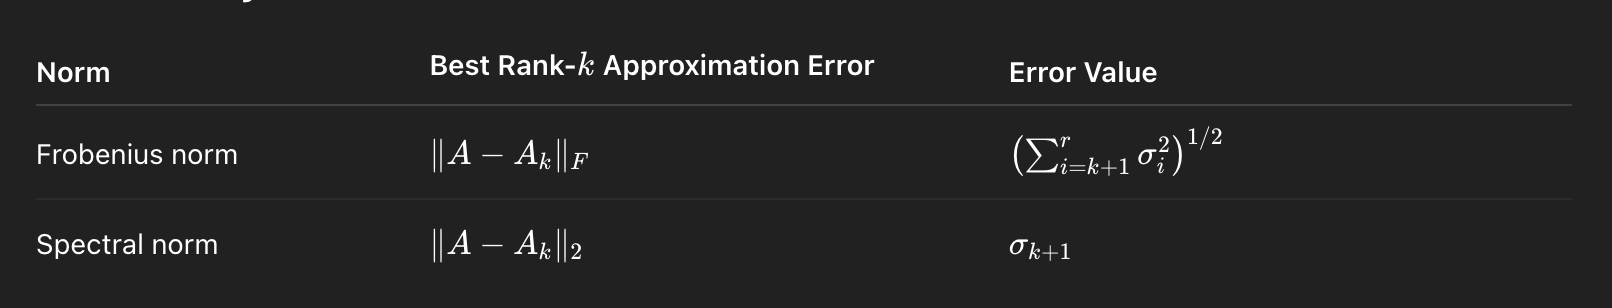
\includegraphics[width=0.7\linewidth]{Figures/Eckart-Young-Theory-reference.png}
            \caption{Summary about Erkart-Young Theory}
            \label{fig:enter-label}
        \end{figure}
    \end{itemize}
\end{itemize}

\subsubsection*{Example: Image Compression}
Code to perform image compression using SVD:
\begin{verbatim}
    using Pkg
    Pkg.add("Images")
    Pkg.add("FileIO")
    Pkg.add("ImageMagick")
    Pkg.add("LinearAlgebra") # for SVD calculations
    Pkg.add("Plots")
    
    using Images, FileIO, LinearAlgebra, Plots

    # This julia file will provide an example of image compression using SVD
    # MUST BE RUN FROM WITHIN THE 'image_compression_example' folder!!
    
    # injesting the image of the dog
    A = load("./Figures/Dog.jpeg")
    
    #turning image into a grey scale image
    gs_A = Gray.(A)
    
    #extracting row and column length from image matrix
    row, col = size(gs_A)[1:2]
    
    U, S , V = svd(gs_A)
    S_diagonal = Diagonal(S)
    
    #Approx A using truncated SVD method
    matrix_rank_truncation_values = [5 20 100]
    
    for r in matrix_rank_truncation_values
      #as the matrix rank increases more detail is added to the final image
      x_approx = U[:, 1:r]*S_diagonal[1:r, 1:r]*transpose(V[:,1:r])
      #creating image
      fname = "./Figures/Truncated_image_rank_$r.png"
      save(fname, heatmap(x_approx))
    end
\end{verbatim}

% Will return to this 

\subsection*{Mathematical Properties and Approximations}

\noindent \textit{This section will cover the important mathematical properties relating to the SVD}

\subsubsection*{Interpretation as Dominant Correlation}

\begin{itemize}
    \item The SVD is closely tied to an eigenvalue problem:
    \begin{itemize}
        \item This eigenvalue problem involves the correlation matrices $XX^*$ (row-wise correlation matrix) and $X^*X$ (column-wise correlation matrix). 
        
        Essentially, the row-wise correlation matrix provides information on how the rows of the matrix are related. This is similar to how a column-wise corelation matrix provides information on how the columns of the matrix are related/are similar to each other. \textit{A correlation matrix can only be determined using a "standardized" (mean-centered and scaled) matrix.}

        The eigenvalues from row-wise correlation matrix shows the maximum variance among rows and the eigenvalues from column-wise correlation matrix shows the maximum variance amongst columns.
        
        \item Solving for $XX^*$:
        \begin{align*}
            XX^* &= U \begin{bmatrix} \hat{\sum} \\
                                    0 
                \end{bmatrix} V^*V \begin{bmatrix}
                    \hat{\sum} & 0
                \end{bmatrix} U^* \\
                &= U \begin{bmatrix}
                    \hat{\sum}^2 & 0 \\
                    0 & 0
                \end{bmatrix} U^* \\
            XX^*U &= U \begin{bmatrix}
                    \hat{\sum}^2 & 0 \\
                    0 & 0
                \end{bmatrix}
        \end{align*}
        \item Solving for $X^*X$:
        \begin{align*}
            X^*X &= V \begin{bmatrix} \hat{\sum} & 0 \end{bmatrix}U^*U \begin{bmatrix} \hat{\sum} \\ 0 \end{bmatrix}V^* \\
                &= V\hat{\sum}^2V^*
            X^*XV &= V\hat{\sum}^2 
        \end{align*}
        \item This analysis shows that each non-zero singular value of X is the positive square root of the eigenvalue of $X^*X$ and $XX^*$ (these two matrices will have the same eigenvalues). Furthermore if $X = X^*$ (aka. the matrix $X$ is self-adjoint) then the singular values will equal the absolute values of the eigenvalues.
        \item Some information on determining Adjoint of a matrix: \href{https://www.youtube.com/watch?v=wjekhHnzL_U}{\textbf{Youtube: Adjoint Matrix}}\newline
        \textit{\textbf{An aside}: Adjoint and Adjugate are many time used interchangeably but in actuality the adjoint involves using the conjugate transpose rather than a regular transpose of the cofactor matrix. \newline The above definition, however, isn't related to the definition of a \href{https://en.wikipedia.org/wiki/Hermitian_matrix}{self-adjoint/Hermitian Matrix}. A self-adjoint matrix is one where $X = X^*$ or in the real space $X = X^T$.}
        \item From this analysis one can also tell that $U$ is the eigenvectors of $XX^*$ and $V$ is the eigenvectors of $X^*X$
        \begin{align*}
            XX^*U &= U\begin{bmatrix} \hat{\sum}^2 & 0 \\ 0 & 0\end{bmatrix}\\
            X^*XV &= V\hat{\sum}^2
        \end{align*}
    \end{itemize}
\end{itemize}

\subsubsection*{Method of Snapshots}

\begin{itemize}
    \item Depending on the problem the state dimension can become very large. The "Method of Snapshots" helps with this problem.
    \begin{itemize}
        \item The trick is to perform eigendecomposition on the $X^*X$ matrix. This would enable one to determine the matrices $V$ and $\hat{\sum}$. If there are zero singular values from the matrix $\hat{\sum}$, then we would keep the $r$ non-zero part (which is the matrix $\tilde{\sum}$ from earlier) and the corresponding columns $\tilde{V}$ of $V$. From this, one can approximate the first r columns of U (which is $\tilde{U}$):
        \begin{equation*}
            \tilde{U} = X\tilde{V}\tilde{\sum}^{-1}
        \end{equation*}
    \end{itemize}
    \item To summarize, the SVD is intimately connected to the \textbf{spectral properties} of the compact self-adjoint matrices
        \begin{itemize}
            \item \textbf{Spectrial properties} of a matrix are the characteristics that relate to its eigenvalues and eigenvectors, which are fundamental in linear algebra and matrix analysis. 
        \end{itemize}
\end{itemize}

\subsubsection*{Generalization of the Eigendecomposition}

\begin{itemize}
    \item The singular value decomposition (SVD) is a generalization of the eigendecomposition of square and defective square matrices. Below is a short explanation of \textbf{defective square matrices}:
    \begin{itemize}
        \item A \textbf{Defective square matrix} is a type of square matrix that does not have a complete basis of vectors. A square matrix is classified as defective when the geometric multiplicity of at least one eigenvalue is less than its algebraic multiplicity.
        \begin{itemize}
            \item \textbf{Algebraic multiplicity}: The number of times an eigenvalue appear as the root of a matrix's characteristic polynomial
            \item \textbf{Geometric multiplicity}: The number of linearly independent eigenvectors associated with an eigenvalue (is equivalent to the dimension of the eigenspace for the eigenvalue).
            \item \textbf{Diagonizability}: A matrix is diagonizable iff the geometric multiplicity of each eigenvalue equals to the algebraic multiplicity and the total number of eigenvectors equals the dimension of the matrix
            \item \textbf{Summary}: Matrix $A$ is defective if there is an eigenvalue ($\lambda$) in which:
            \begin{equation*}
                \text{Geometric Multiplicity of $\lambda$} < \text{Algebraic Multiplicity of $\lambda$}
            \end{equation*}
        \end{itemize}
        \item Eigendecomposition of regular diagonalizable square matrix $X$:
        \begin{equation*}
            XV = V\Lambda \Rightarrow X = V\Lambda V^{-1}
        \end{equation*}
        \textit{The thing to note is that matrix $V$ is not a unitary matrix, therefore $V^* \neq V^{-1}$}
        \item Eigendecomposition of a Hermitian Matrix (self-adjoint matrix) where $X = X^*$
        \begin{equation*}
            XV = V\Lambda \Rightarrow X = V\Lambda V^{*}
        \end{equation*}
        \textit{Here, matrix $V$ is a unitary matrix, therefore $V^{-1} = V^*$}
        \item The SVD can be written in a similar form to the above representations:
        \begin{equation*}
            XV = U\sum \Rightarrow X = U\sum V^*
        \end{equation*}
    \end{itemize}
\end{itemize}

\subsubsection*{Geometric Interpretations}

\begin{itemize}
    \item When performing SVD, the columns of the matrix $U$ is orthonormal to the columns of $X$ and the columns of matrix $V$ is orthonormal to the rows of $X$.
    \begin{itemize}
        \item \textbf{What are orthonormal vectors (for my review :))?:} These are vectors that are orthogonal to each other (dot product = 0), and the vectors have unit mangitude (the magnitude of the vectors are equal to 1).
    \end{itemize}
\end{itemize}

\subsubsection*{Invariance of the SVD to Unitary Transformations}

\begin{itemize}
    \item A interesting, yet useful, property of SVD is when you perform a left or right unitary transformation (an example is discrete fourier transform, or $\mathbb{F}$) to either the $U$ or $V$ matrices, it does not impact the terms in the SVD.
    \item This invariance is attributed to the fact that unitary transformation only rotate a vector but do not move its inner product (aka. dot product)
    \begin{itemize}
        \item \textit{Page 16 in the textbook shows examples of left and right unitary transformations}
    \end{itemize}
\end{itemize}

\subsection*{Pseudo-inverse, Least squares, and Regression}

\begin{itemize}
    \item Basic information on systems of linear equations written in matrix form
    \begin{equation*}
        Ax = b
    \end{equation*}
    \begin{itemize}
        \item If $A$ is a square and invertible matrix, then there is a single solution $x$ for every $b$ where $x=A^{-1}b$. If matrix $A$ is rectangular or singular, then you could also end up with infinite solutions, or no solutions. Usually \textbf{under-determined systems} have infinite solutions, while \textbf{over-determined systems} have no solution.
        \begin{itemize}
            \item \textit{A singular matrix is a square matrix with a determinant equal to 0 (therefore, it can't be inverted)}
        \end{itemize}
    \end{itemize}
    \item Other information to understand from basic linear algebra:
    \begin{itemize}
        \item The \textbf{column space} of matrix $A$ is the \textbf{span} of the columns of the columns of $A$. The \textbf{span} is the number of linearly independent vectors. The \textbf{column space} is also known as the \textbf{range}.
        \begin{itemize}
            \item In SVD, the column space of $A$ in the equation $A = \tilde{U}\tilde{\sum}\tilde{V}^*$ is equal to the column space of $\tilde{U}$ where $\tilde{U}$ is a truncated version of $U$ based on the rank of $X$.
            \item The orthogonal complement to the $col(A)$ is $ker(A^*)$ and is given by the column space of $\hat U^\perp$.
        \end{itemize}

        \item The \textbf{row space} of $A$ is the span of the rows of $A$ ($\text{row}(A) = \text{col}(A^*)$). \newline
        \begin{itemize}
            \item In SVD, the row space of $A$ (where $A = \tilde{U}\tilde{\sum}\tilde{V}^*$), is equal to the row space of $\tilde{V}^*$ or the column space of $\tilde{V}$. Similarly, $\tilde{V}$ is a truncated version of $V$ based on the rank of $X$.
            \item the orthogonal complement of $row(A)$ is $ker(A)$ (null space) and is derived from $col(\hat V^\perp$
        \end{itemize}

        \item to summarize, if $b \in col(A)$ and $dim(ker(A)) \neq 0$ then there is an infinite number of solutions, $x$. If $b \notin col(A)$ then there are no solutions. 
        
        \textbf{Essentially, the $dim(ker(A))$ is the NUMBER OF FREE VARIABLES! So if $dim(ker(A))$ is positive, then the number of equations is less than the number of unknowns.}

        \item The fundamental subspaces follow the following equations:
        \begin{align*}
            col(A) \oplus ker(A^*) = \mathbb{R}^n \\
            col(A^*) \oplus ker(A) = \mathbb{R}^n
        \end{align*}
    \end{itemize}
\end{itemize}

\subsubsection*{Condition Number}

\begin{itemize}
    \item What is the \textbf{condition number?}:
    \begin{itemize}
        \item represents how sensitive matrix multiplication and matrix inversion are to changes to the input \textit{(useful information in APC - Advanced Process Control - development)}.
        \item Equation to calculate the condition number:
        \begin{equation*}
            \kappa(A) = \frac{\sigma_{max}(A)}{\sigma_{min}(A)}
        \end{equation*}
        Where,
        \begin{conditions}
            \kappa & Condition number \\
            \sigma_{max} & Max singular value \\
            \sigma_{min} & Min singular value \\
            A & Input matrix
        \end{conditions}
        \item in APC development conditions value analysis is used in determining colinearities within the RGA (relative gain array). Near colinearities or colinearities can cause cycling to occur within a MPC (model predictive controller) and thus can cause equipment damage at a plant.
    \end{itemize}
    \item How does one illustrate the effect of a large condition value:
    \begin{itemize}
        \item If you are apply error margins to the equation $Ax = b$ one gets the following equation:
        \begin{equation*}
            A(x + \epsilon_x) = b + \epsilon_b
        \end{equation*}
        \item If we assume a worst case scenario where $\epsilon_x$ is aligned with the max singular value, $\sigma_{max}$, and the input, $x$, is aligned with the minimum singular value, $\sigma_{min}$, one will get the following equation:
        \begin{equation*}
            A(x + \epsilon_x) = \sigma_{min}x + \sigma_{max}\epsilon_x
        \end{equation*}
        Where,
        \begin{conditions}
            \sigma_{min}x & $b$ \\
            \sigma_{max}\epsilon_x & $\epsilon_b$
        \end{conditions}
        \item From the above equation, the output signal-to-noise ratio ($\frac{b}{\epsilon_b}$) is equal to $\frac{x}{\epsilon_x} \cdot \frac{\sigma_{min}}{\sigma_{max}}$ 
    \end{itemize}
    \item One approach to mitigating a large condition number is to truncate the SVD more aggressively; however, this comes at the cost of decreasing the size of the subspace $\tilde{U}$ which is used to approximate the output. In other words, by performing an aggressive truncation, the approximate result (that one would get from the aggressive truncation of SVD) may lose important information of the higher dimensional system and therefore would not be a good model to represent the higher dimensional system.
\end{itemize}

\subsubsection*{One-Dimensional Linear Regression}

\begin{itemize}
    \item Regressions are important to understand how one variable relates to another, if any exists. SVD is a method to solve a linear system of equations (such as $Ax=b$) particularly when $A$ isn't square or full-rank
    \item Example:
    \begin{itemize}
        \item One can use a pseudo inverse to determine the least-squares solution, as shown in the equation below:
        \begin{align*}
            b &= ax = \tilde{U}\tilde{\sum}\tilde{V}^*x \\
            x &= \tilde{V}\tilde{\sum}^{-1}\tilde{U}^*b
        \end{align*}
        Where,
        \begin{conditions}
            \tilde{\sum} & $\Vert a \Vert_2$ \\
            \tilde{U} & $\frac{a}{\Vert a \Vert_2}$ \\
            \tilde{V} & 1
        \end{conditions}
        \item Taking the pseudo-inverse, we get the following equation:
        \begin{equation*}
            x = \frac{a^*\cdot b}{\Vert a \Vert_2^2}
        \end{equation*}
    \end{itemize}
    \item \textit{Interesting things happen if $a$ is a row vector rather than column vector}
    \begin{itemize}
        \item \textbf{What if $a$ is row vector (information provided by ChatGPT!)}: \newline

        If \( a \) is a **row vector** instead of a column vector, the concept of the Singular Value Decomposition (SVD) still applies, but we need to make some adjustments for the specific case where \( M = a \) is a row vector.

Let’s walk through this step by step.

---

### **1. Matrix \( M \) as a Row Vector:**

Now, suppose \( M \) is a \( 1 \times n \) **row vector**:
\[
M = \begin{bmatrix} a_1 & a_2 & \dots & a_n \end{bmatrix}.
\]

This is different from the previous case where \( a \) was a column vector.

---

### **2. SVD for a Row Vector:**

For a row vector \( M \), the SVD is:
\[
M = U \Sigma V^T,
\]
where:
- \( U \) is an orthogonal matrix (containing the left singular vectors),
- \( \Sigma \) is a diagonal matrix (containing the singular values),
- \( V \) is an orthogonal matrix (containing the right singular vectors).

In the case of a \( 1 \times n \) row vector, \( M \) has a single nonzero singular value, corresponding to the nonzero eigenvalue of \( M^T M \).

---

### **3. Compute \( M^T M \):**

To understand how the SVD works, let’s start by computing \( M^T M \), which is the matrix involved in finding the right singular vectors in \( V \).

- If \( M \) is a row vector of size \( 1 \times n \), then \( M^T \) is an \( n \times 1 \) column vector.
- So, \( M^T M \) is an \( n \times n \) matrix:
\[
M^T M = \begin{bmatrix} a_1 \\ a_2 \\ \dots \\ a_n \end{bmatrix} \begin{bmatrix} a_1 & a_2 & \dots & a_n \end{bmatrix} = \begin{bmatrix} a_1^2 & a_1 a_2 & \dots & a_1 a_n \\ a_2 a_1 & a_2^2 & \dots & a_2 a_n \\ \vdots & \vdots & \ddots & \vdots \\ a_n a_1 & a_n a_2 & \dots & a_n^2 \end{bmatrix}.
\]

This is an \( n \times n \) **rank-1** matrix, just like the case where \( a \) was a column vector. The eigenvalue decomposition of \( M^T M \) will give us the right singular vectors in \( V \).

---

### **4. Eigenvalue Decomposition of \( M^T M \):**

- Since \( M^T M \) is a rank-1 matrix, it has **one nonzero eigenvalue**, which is:
  \[
  \lambda = \|a\|_2^2 = \sum_{i=1}^n a_i^2.
  \]

- The eigenvector corresponding to this nonzero eigenvalue is the normalized version of the row vector \( a \):
  \[
  v_1 = \frac{a^T}{\|a\|_2}.
  \]

- The other \( n-1 \) eigenvectors of \( M^T M \) are orthogonal to \( v_1 \) and correspond to the zero eigenvalues. These can be any orthonormal vectors in the null space of \( M^T M \).

Thus, \( V \), the matrix of right singular vectors, will have:
- The first column \( v_1 = \frac{a^T}{\|a\|_2} \),
- The remaining columns are orthonormal vectors corresponding to the zero eigenvalues.

---

### **5. Compute \( MM^T \):**

Next, we compute \( MM^T \), which will give us the left singular vectors \( U \).

- \( M \) is a \( 1 \times n \) row vector, so \( MM^T \) is a \( 1 \times 1 \) scalar matrix:
\[
MM^T = a a^T = \|a\|_2^2.
\]

This is just a scalar (the squared \( \ell_2 \)-norm of \( a \)).

- The eigenvector corresponding to this eigenvalue is simply \( u_1 = 1 \) (since it's a \( 1 \times 1 \) matrix).

Thus, in this case, the matrix \( U \) is a \( 1 \times 1 \) matrix, which is just the scalar \( 1 \).

---

### **6. Singular Values:**

The singular values are the square roots of the eigenvalues of \( M^T M \) (or \( MM^T \), since they are the same in this case). The nonzero singular value is:
\[
\sigma = \|a\|_2.
\]

Thus, the matrix \( \Sigma \) will have the singular value \( \|a\|_2 \) on the diagonal, and all other values will be zero.

---

### **Summary for Row Vector \( a \):**

- \( M = a \) is a row vector \( 1 \times n \).
- The **right singular vectors** (columns of \( V \)) are:
  - The first column of \( V \), \( v_1 = \frac{a^T}{\|a\|_2} \), corresponds to the eigenvector of \( M^T M \).
  - The remaining columns of \( V \) are orthonormal vectors corresponding to the zero eigenvalues of \( M^T M \).
  
- The **left singular vector** \( U \) is a \( 1 \times 1 \) matrix (since \( MM^T \) is a scalar), and it is just \( 1 \).

    \end{itemize}
\end{itemize}

\subsubsection*{Multi-linear Regression}

\begin{itemize}
    \item \textit{This section of the textbook provides Matlab examples which are good to do in Julia lang} 
\end{itemize}

\subsection*{Principle Component Analysis (PCA)}

\begin{itemize}
    \item What is Principle Component Analysis?
    \begin{itemize}
        \item Provides a statistical interpretation of the coordinate system used to represent the high-dimensional correlated data. The coordinate system involves the use of the correlation matrices (the $XX^*$ and $X^*X$ matrices)
        \begin{itemize}
            \item \textbf{From ChatGPT:} PCA seeks to transform the data into a coordinate system where the axes are the Principle components which are aligned with directions of maximum variance. The PCs themselves are linear combinations of the original variables that make up the data.
        \end{itemize}
        \item The geometry of the coordinate system is determined using \textbf{Principle Components (PCs)} that are orthogonal to each other but have a maximal correlation with the measurements.
        \item \textbf{From Chat GPT:} PCA transforms this high-dimensional space into a new coordinate system where the axes are the principal components. These new axes are linear combinations of the original features that capture the directions of maximum variance. The PCs provide information on the pattern and structures within the data, many times not directly observable in high dimensional data.
        \item PCA generally uses SVD to perform its calculations \textit{(Referred as the PCA/SVD technique)}.
    \end{itemize}
\end{itemize}

\subsubsection*{Computation}

\begin{itemize}
    \item Process for PCA for experiments:
    \begin{enumerate}
        \item A large number of experiments are taken, with each measurement vector representing a row within the matrix $X$. \textit{This differs from other types of analysis methods where individual features maybe represented as columns in matrix $X$. This methodology of PCA, as discussed in this section of the notes, is aligned with the literature.}
        \item Once the data collection has happened, the average row is computed ($\Bar{x}$)
        \begin{equation*}
            \Bar{x}_j = \frac{1}{n}\sum_{i=1}^n X_{ij}
        \end{equation*}
        \item from the $\Bar{x}$ one can determine the mean matrix frrom the following:
        \begin{equation*}
            \Bar{X} = \begin{bmatrix}
                1 \\
                \vdots \\
                1
            \end{bmatrix} \Bar{x}
        \end{equation*}
        \item next, the mean-subtracted matrix, $B$, can be determined which is then used to determine the covariance matrix, $C$:
        \begin{equation*}
            B = X - \Bar{X}
        \end{equation*}
        \begin{equation*}
            C = \frac{1}{n-1}B^*B
        \end{equation*}

        \textit{The reason we use $n-1$ (known as \textbf{Bessel's Correction}) is because the above steps to determine the sample variance does not account for the variance of $\Bar{X}$ (sample mean) against the true mean.}

        \textit{\textbf{From ChatGPT:} Bessel's correction refers to the adjustment made to the calculation of the sample variance or standard deviation to account for the fact that using the sample mean instead of the population mean underestimates the variability in the data.}

        \item The PCs (principle components) are the eigenvectors of $C$ and they define a change in coordinates.
        \begin{equation*}
            CV = VD \Rightarrow C = VDV^* \Rightarrow D = V^*CV
        \end{equation*}

        Plugging the equation above related $B$ to $C$ and using SVD $B = U\sum V^*$, one can derive the following:
        \begin{align*}
            C &= \frac{1}{n-1}B^*B \\
            &= \frac{1}{n-1}V\left(\sum \right)^2V^* \\
            D &= \frac{1}{n-1}\left(\sum \right)^2
        \end{align*}

        One can relate the singular values to the singular values to the eigenvalues using the following equation:
        \begin{equation*}
            \lambda_k = \frac{\sigma_k^2}{n-1}
        \end{equation*}


        \textit{\textbf{From ChatGPT:} Principal components are the new variables that are formed as linear combinations of the original variables in a dataset. These components aim to capture the maximum variability in the data, making them the most informative features for analysis and dimensionality reduction.}
        
        \begin{itemize}
            \item Properties of Principle Components \textbf{(From ChatGPT)}:
            \begin{itemize}
                \item Orthogonality
                \item Order of variance -> The principle components are ordered from greatest to least variance.
                \item PCs are the eigenvectors of the covariance matrix
                \item the eigenvalues represent the variance for each PC.
            \end{itemize}
        \end{itemize}
    \end{enumerate}
\end{itemize}

\subsection*{Eigenface Example}
\textit{This is an example of PCA/SVD... need to return to this}

\subsection*{Truncation and Alignment}

\begin{itemize}
    \item Determine number of singular values to keep is a debated topic. One approach involves predetermining the amount of variance in the original data (such as 90 or 99\% truncation). Another approach is determining "elbows" or "knees" in the SVD. This is when the singular values transition from representing the important patterns to noise. However, both of these methods have their limitations.
\end{itemize}

\subsubsection*{Optimal Hard Threshold}

\begin{itemize}
    \item In matrices that have a low rank and contain "Gaussian white noise", one can determine a \textbf{optimal hard threshold, $\tau$,} for singular value truncation
    \item How does this work?:
    \begin{enumerate}
        \item Start with the assumption that matrix $X$ is made up of a low rank matrix $X_{\text{true}}$ and noise matrix $X_{\text{noise}}$ through the following equation:
        \begin{equation*}
            X = X_{\text{true}} + \gamma X_{\text{noise}}
        \end{equation*}
        Where,
        \begin{conditions}
            \gamma & The magnitude of the Gaussian white noise
        \end{conditions}
        \item If $\gamma$ is known, then $\tau$ (the optimal hard threshold) can be determined through the following equations:
        \begin{itemize}
            \item If $X \in R^{n \cdot n}$ (matrix $X$ is square):
            \begin{equation*}
                \tau = \left( \frac{4}{\sqrt{3}}\right)\sqrt{n}\gamma
            \end{equation*}
            \item If $X \in R^{n \cdot m}$ (matrix $X$ is rectangular):
            \begin{equation*}
                \tau = \lambda(\beta)\sqrt{n}\gamma
            \end{equation*}
            Where,
            \begin{equation*}
                \lambda(\beta) = \left( 2(\beta + 1) + \frac{8\beta}{(\beta + 1) + (\beta^2 + 14\beta + 1)^{\frac{1}{2}}} \right)^{\frac{1}{2}}
            \end{equation*}
            \begin{itemize}
                \item \textit{When $m << n$ then $\beta = \frac{m}{n}$}
                \item \textit{When $n << m$ then $\beta = \frac{n}{m}$}
            \end{itemize}
        \end{itemize}
    \end{enumerate}
\end{itemize}

\textit{Look into Example Problems here --> Page 36 in textbook}

\subsubsection*{Importance of Data Alignment}

\begin{itemize}
    \item An important thing to note about SVD is that it is \textbf{fundamentally geometric}. 
    
    In other words, rotating, stretching, compressing, or translating the vectors in matrix $X$ (with regards to the equation $X = U\sum V^*$) impacts the matrices $U$, $\sum$, and $V$. Specifically, rotations can impact the left and right singular matrices ($U$ and $V$ respectively), while stretching or compressing (changing the magnitude) the vectors of matrix $X$ can cause changes to $\sum$.

    \item Because SVD is sensitive to the alignment of the data, SVD can't be used on data that hasn't been heavily preprocessed.
\end{itemize}

\subsection*{Randomized Singular Value Decomposition}

\textbf{Thing to Note: }The use of \textbf{Randomized numerical methods} have the potential to provide accurate matrix decompositions at a fraction of the computational cost. This will be more important in the future as it has been shown that, in most cases, while the rank of the measurement space can grow, the intrinsic rank doesn't increase proportionally.

\subsubsection*{Randomized Linear Algebra}

\begin{itemize}
    \item Steps for Randomized Linear Algebra (specific to SVD). This works primarily for \textbf{tall-skinny matrices}, where $n < m$ or number of rows, $n$, are greater than number of columns, $m$.
    \begin{enumerate}
        \item Identify a target rank, where $r < m$. \newline
        \textit{\textbf{Note:} The "rank" is the dimension of the column space.}

        \item Use random projections, $P$, to sample the column space and find a matrix $Q$ that can approximate the column space of $X$, so that $X \approx QQ^*X$ \textit{<-- Here one is using column based projection}

        \item Project $X$ onto $Q$ subspace ($Y = Q^*X$) and compute the matrix decomposition on $Y$. \newline
        \textbf{Notes on what "project"/projection refers to:}
        \begin{itemize}
            \item In projection, one can either project each column of matrix $A$ onto the column space of matrix $B$ or one can project the rows of $A$ onto the row space of matrix $B$.
            \begin{itemize}
                \item Column Space Projection Equation ($A$ onto $B$):
                \begin{equation*}
                    proj_B(A) = B(B^TB)^{-1}B^TA                
                \end{equation*}
                \item Row Space Projection Equation ($A$ onto $B$):
                \begin{equation*}
                    proj_B(A) = AB^T(BB^T)^{-1}                
                \end{equation*}
            \end{itemize}
        \end{itemize}

        \item Reconstruct high-dimensional modes $U = QU_Y$ using Q and the modes computed from $Y$. \newline
        \textit{\textbf{Note:} Mode refers to different dimensions or axes}
    \end{enumerate}
\end{itemize}

\subsubsection*{Randomized SVD algorithm}

\begin{itemize}
    \item Steps:
    \begin{enumerate}
        \item Construct a projection matrix, $P \in R^{m\cdot r}$, to sample the column space of matrix $X$, where $X \in R^{n \cdot m}$.
        \begin{equation*}
            Z = XP
        \end{equation*}

        \textit{\textbf{Note:} For low rank matrices and where $r << m$, $Z$ might be smaller than $X$. This is because a random projection matrix might not capture the important components from $X$ and as a result, $Z$ approximates the column vectors of $X$ with high probability. This can be helpful in determining a $QR$ decomposition for $Z$ to find the orthonormal basis for $X$.}

        \item With a low rank basis $Q$, one can project $X$ into smaller spaces.
        \begin{equation*}
            Y = Q^*X
        \end{equation*}

        \textit{\textbf{Note:} It stands to reason that $X \approx QY$ especially in cases when $\sigma_k$ is decaying (when $k > r$). This is because at lower singular values represent noise in the system and a result, a small change in the input vector (right singular vector) does not create a significant change in the left singular vector.}

        Once one determines $Y$, one can perform SVD on $Y$:
        \begin{equation*}
            Y = U_Y\sum V^*
        \end{equation*}
        
        \item Using $U_Y$ and $Q$, one can determine the high-dimensional left singular vectors, $U$.
        \begin{equation*}
            U = QU_Y    
        \end{equation*}
    \end{enumerate}
    \item Figure of Randomized SVD algorithm:
    \begin{figure}[hbt!]
        \centering
        \includegraphics[width=0.5\linewidth]{Figures/Randomized_SVD_fig.png}
        \caption{Process of Randomized SVD using the Halko, Martinsson, and Tropp algorithm}
        \label{fig:Randomized-SVD}
    \end{figure}

    \item \textit{\textbf{Note:} A \textbf{randomized projection matrix} is a matrix, \( P \), with random entries (often drawn from a Gaussian distribution) that is used to project a large matrix, \( X \), onto a lower-dimensional subspace. The goal is to capture the most significant features of \( X \), such as its dominant singular values and vectors, with fewer computational resources. By multiplying \( X \) with \( P \), we obtain a smaller matrix, \( Y = XP \), that retains the essential structure of \( X \), enabling efficient approximation of its singular value decomposition (SVD).}    
    
    \item \textit{\textbf{Note:}\href{https://tropp.caltech.edu/slides/Tro21-RandSVD-slides.pdf}{Link to more relevant information on SVD}}
\end{itemize}

\subsubsection*{Oversampling}

\begin{itemize}
    \item In case (which is most of the time) when $X$ is not a low-rank matrix, there will be non-zero singular values, $\sigma_k$ when $k > r$. One can increase the columns of the randomized projection matrix ($P$) to reduce variance in the singular values, a method called \textbf{oversampling}. 
    \item This method is important so that matrix $Y$ can hold the dominant components (components with the most information) from the original matrix.
\end{itemize}

\subsubsection*{Power Iterations}

\begin{itemize}
    \item Another challenge with the SVD is when there is a slow decay in the singular values. In this situation, one can utilize \textbf{q power iterations} to create a new matrix, $X^{(q)}$, that has more rapid singular value decay.
    \begin{equation*}
        X^{(q)} = (XX^*)^qX
    \end{equation*}
    \item The Downside is that the power iterations are expensive as it requires $q$ passes at matrix $X$
\end{itemize}

\subsubsection*{Guaranteed Error Bounds}

\begin{itemize}
    \item In a deterministic algorithm, one can define the error through the following equation:
    \begin{equation*}
        \Vert X - QY \Vert_2 \geq \sigma_{r+1}(X)
    \end{equation*}
    \item In a randomized algorithm, one can determine the \textbf{expected error}:
    \begin{equation*}
        \mathbb{E}(\Vert X - QY \Vert_2) \leq \left( 1 + \sqrt{\frac{r}{p-1}} + \frac{e\sqrt{r+p}}{p}\sqrt{m-r} \right)^{1/(2q+1)}\sigma_{k+1}(X)
    \end{equation*}
    Where,
    \begin{conditions}
        e & Euler number
    \end{conditions}
\end{itemize}

\subsubsection*{Choice of Random Matrix $P$}

\begin{itemize}
    \item What are some choices for the random matrix, $P$:
    \begin{enumerate}
        \item \textbf{Gaussian Random Projections} are used frequently due to favorable mathematical properties and the richness of information extracted. However, Gaussian Random Projections are hard to generate, store, and compute. \textbf{Uniform random matrices} are also used frequently and have similar limitations.
        \item \textbf{Structured Random Projections} can also provide efficient sketches and bring down computational costs to $\mathbb{O}(nm\text{log}(r))$
        \item Another example are \textbf{Rademacher matrices} where entries can be $+1$ or $-1$ of equal probability.
        \item An extreme option is randomly choosing columns of $X$ for the sketch $Z$. This is risky as the important columns of $X$ could be localized to a particular region.
    \end{enumerate}
\end{itemize}

\textit{Look into Randomized SVD example here --> Page 44}

\subsection*{Tensor Decomposition and N-Way Data Arrays}

\begin{itemize}
    \item The purpose of N-ways arrays or tensors is to preserve the data structures and types in their own independent directions without forcing a data flattening process.
    \item The development of data tensors requires one to revisit tensor addition, multiplication, and inner products
    \begin{enumerate}
        \item First we denote the $r^{th}$ column of matrix $A$ as $a_r$.
        \item Say that we have two matrices: $A \in \mathbb{R}^{\mathbb{I}\times \mathbb{K}}$ and $B \in \mathbb{R}^{\mathbb{J}\times \mathbb{K}}$. Their \textbf{Khatri-Rao product} is denoted by $A 
        \odot B$
        \begin{itemize}
            \item The \textbf{Khatri-Rao product} is a column-wise \textbf{Kronecker product} of 2 matrices with the same number of columns. This is represented by the following equation:
            \begin{equation*}
                A \odot B = (a_1 \otimes b_1 \cdots a_K \otimes b_K)
            \end{equation*}
            \textit{Where the subscript number in the above formula represents the column number.}
            \item The \textbf{Kronecker product} is a tensor product on two matrices to produce a larger matrix. It is denoted by the symbol $\otimes$.

            Mathematically, for \( A = [a_{ij}] \) and \( B = [b_{kl}] \), the Kronecker product is:

            \[
            A \otimes B = 
            \begin{bmatrix}
            a_{11}B & a_{12}B & \dots & a_{1n}B \\
            a_{21}B & a_{22}B & \dots & a_{2n}B \\
            \vdots & \vdots & \ddots & \vdots \\
            a_{m1}B & a_{m2}B & \dots & a_{mn}B
            \end{bmatrix}
            \]
            
            \textbf{Example:}
            
            Let
            \[
            A = \begin{bmatrix} 1 & 2 \\ 3 & 4 \end{bmatrix}, \quad B = \begin{bmatrix} 0 & 5 \\ 6 & 7 \end{bmatrix}
            \]
            The Kronecker product \( A \otimes B \) is calculated as:
            
            \[
            A \otimes B = \begin{bmatrix}
            1 \cdot B & 2 \cdot B \\
            3 \cdot B & 4 \cdot B
            \end{bmatrix}
            = \begin{bmatrix}
            \begin{bmatrix} 0 & 5 \\ 6 & 7 \end{bmatrix} & \begin{bmatrix} 0 & 10 \\ 12 & 14 \end{bmatrix} \\
            \begin{bmatrix} 0 & 5 \\ 6 & 7 \end{bmatrix} \cdot 3 & \begin{bmatrix} 0 & 5 \\ 6 & 7 \end{bmatrix} \cdot 4
            \end{bmatrix}
            = \begin{bmatrix}
            0 & 5 & 0 & 10 \\
            6 & 7 & 12 & 14 \\
            0 & 15 & 0 & 20 \\
            18 & 21 & 24 & 28
            \end{bmatrix}
            \]
        \end{itemize}
        
        \item The inner product of two N-way tensors (for example, $\mathbb{A}$ and $\mathbb{B}$) is shown below
        \begin{equation*}
            \left < \mathbb{A}, \mathbb{B}\right> = \sum_i a_ib_i
        \end{equation*}
        Where: $\mathbb{A}$ is of size $I_1\times I_2 \times \cdots \times I_N$ and $i = (i_1, i_2, \cdots, i_n)$

        \item The Frobenius norm of a tensor A (denoted as $\Vert \mathbb{A} \Vert_F$) is the square root of the inner product (aka. dot product).
        \begin{equation*}
            \Vert \mathbb{A} \Vert_F = \sqrt{\left< \mathbb{A}, \mathbb{A}\right>}
        \end{equation*}

        \textit{Below are some more information about inner and outer products:}
        \begin{itemize}
            \item inner product (aka. dot product) is represented by the following equation:
            \begin{equation*}
                a \cdot b = a^Tb
            \end{equation*}
            \item the outer product is represented by the following equation:
            \begin{equation*}
                a\cdot b = ab^T
            \end{equation*}
            
            where, $a = \left[a_1, a_2, a_3, \cdots, a_n\right]$ and $b = \left[ b_1, b_2, b_3, \cdots, b_n\right] $
        \end{itemize}

        \item The mode-n matricization (or unfolding of tensor $\mathbb{A}$) is denoted by $mA_{(n)}$
    \end{enumerate}
    \item How to formulate a N-ways data array?:
    \begin{enumerate}
        \item If we are representing $\mathbb{M}$ as a tensor of size $I_1 \times I_2 \times \cdots \times I_N$, we can develop a \textbf{R-component CANDECOMP/PARAFAC (CP) factor model}
        \begin{itemize}
            \item the meaning of $I_1 \times I_2 \times \cdots \times I_N$ is to represent the number of modes (aka. dimensions) of the tensor
            \item the \textbf{CANDECOMP/PARAFAC (CP)} decomposition is a way to express a tensor as a sum of rank-one tensors.
            \begin{equation*}
                \mathcal{X} = \sum^R_{r=1}  a_r \circ b_r \circ c_r
            \end{equation*}
            Where $A \in \mathbb{R}^{I_1\times R}$, $B \in \mathbb{R}^{I_2\times R}$, and $C \in \mathbb{R}^{I_3\times R}$

            The R-component in CP decomposition refers to the decomposition of the tensor to the R$^{\text{th}}$ factor matrix.
        \end{itemize}
        \item the overall equation is the following:
        \begin{equation*}
            \mathbb{M} = \sum^R_{r=1} \lambda_r ma_r^{(1)} \circ ma_r^{(2)} \circ \cdots \circ ma_r^{(N)}
        \end{equation*}
        where 
        \begin{conditions}
            \circ & outer product \\
            ma_r^{(n)} & rth column of the factor matrix of $mA^{(n)}$ of size $I_n \times R$ \\
            \lambda_r & The weight, where $\lambda = (\lambda_1, \lambda_2, \cdots, \lambda_R)^T$ (assuming column normalized to Euclidean length).
        \end{conditions}
    \end{enumerate}
    \item Example:
        \begin{figure}[hbt!]
            \centering
            \includegraphics[width=0.5\linewidth]{Figures/Compare_SVD_to_tensor_decomp.png}
            \caption{Comparison of SVD to Tensor Decomposition of N-ways Data Array}
            \label{fig:Compare_SVD_to_Tensor_Decomp}
        \end{figure}
\end{itemize}

\section{Fourier \& Wavelet Transforms}

\subsection*{Fourier Series and Fourier Transforms}

\begin{itemize}
    \item Fourier Transform decomposing PDEs are analogous to SVD decomposing high-dimensional matrices
    \item The Fourier transform and Fourier series are closely related to the geometry of \textbf{hilbert spaces} (infinite-dimensional function spaces), which generalize vector spaces to include functions that contain infinitely many degrees of freedom (aka. \textbf{function spaces)}.
    \begin{itemize}
        \item \textbf{Note:} A \textbf{\href{https://en.wikipedia.org/wiki/Hilbert_space}{Hilbert space}} is a complete vector space that is equipped with an inner product. Hilbert spaces were originally used to study finite-dimensional vector spaces but have been expanded to study function spaces (essentially vector spaces of infinite dimension).
        \item \textbf{Information from Chat GPT: }An inner product space is a vector space $V$ over $\mathbb{R}$ or $\mathbb{C}$ with a function $\langle \cdot, \cdot \rangle : V \times V \to \mathbb{F}$ (where $\mathbb{F}$ is either $\mathbb{R}$ or $\mathbb{C}$) called an inner product, satisfying the following properties for all $x, y, z \in V$ and scalars $\alpha$.
        \item \textbf{Information from Claude: }A complete space is one where all Cauchy sequences converge to a value within the space.
    \end{itemize}
\end{itemize}

\subsubsection*{Inner products of functions and vectors}

\begin{itemize}
    \item How to determine the Hermitian inner product of the functions $f(x)$ and $g(x)$
    \begin{equation*}
        \left<f(x), g(x) \right> = \int_a^b f(x)\Bar{g}(x)dx
    \end{equation*}
    where $\Bar{g}(x)$ is the complex conjugate of $g(x)$
    
    \item because the magnitude of the inner product increases as number of data points to the vector increases, a normalization parameter $\frac{b-a}{n-1}$ is added:
    \begin{equation*}
        \frac{b-a}{n-1}\left<f(x), g(x) \right> = \sum_{k=1}^n f(x_k)\Bar{g}(x_k)\Delta x
    \end{equation*}
    where $b = x_n$ and $a = x_1$. The above equation is also a Reimann approximation of the continuous functions. As $\Delta x \rightarrow \infty$ the approximate will equal the exact result.

    \item One can also determine the norm of a function (ex provided is the 2-norm):
    \begin{equation*}
        \Vert f \Vert_2 = \sqrt{\left<f,f\right>} = \left(\int_a^b f(x)\Bar{f}(x)dx\right)^{1/2} =\left(\int_a^b |f(x)|^2dx\right)^{1/2} 
    \end{equation*}

    A generalization of the above equation for $L^{p}$-norms:
    \begin{equation*}
        \Vert f \Vert_p = \left(\int_a^b |f(x)|^p dx\right)^{1/p} = \left(\int_a^b (f(x)\Bar{f}(x))^{p/2} dx\right)^{1/p}
    \end{equation*}

    \item The set of all functions with bounded norm defines the set of \textbf{square integrable functions}($L^2$) also known as the \textbf{Lebesque integrable functions}
    \begin{itemize}
        \item A bounded norm is where the norm is less than infinity. An example with the 2-norm is shown below:
        \begin{equation*}
            \Vert f \Vert_2 < \infty
        \end{equation*}
        We can also state that square-integrable functions are functions where the integral of the square is finite. In other words, the function does not \textbf{grow too quickly} as it approaches infinity.
    \end{itemize}

    \item Similarly to finite-dimensional vector spaces, the inner product can be used to project a function into a new coordinate system using orthogonal functions. The \textbf{Fourier series} is an example of a \textbf{projection} of function $f$ onto an orthogonal set of sine and cosine.
\end{itemize}

\subsubsection*{Fourier Series}

\begin{itemize}
    \item The core principle of the Fourier series is that if $f(x)$ is periodic and piecewise smooth, then it can be written as a series of sine and cosine functions with increasing frequency.
    \begin{itemize}
        \item The Fourier series uses the Lebesque integrable functions over the range of $-\pi$ to $\pi$ (in other words, $L^2[-\pi, \pi]$). 
    \end{itemize}
    \item Example: If $f(x)$ is $2\pi$-periodic, it can be written as:
    \begin{equation*}
        f(x) = \frac{a_0}{2} + \sum^\infty_{k=1} (a_kcos(kx)+ b_ksin(kx))
    \end{equation*}
    Where:
    \begin{equation*}
        a_k = \frac{1}{\pi}\int^\pi_{-\pi}f(x)cos(kx) dx
    \end{equation*}
    \begin{equation*}
        b_k = \frac{1}{\pi}\int^\pi_{-\pi}f(x)sin(kx) dx
    \end{equation*}
    $a_k$ and $b_k$ can be viewed as the coordinates from projecting the function, $f(x)$, onto the orthogonal sine and cosine basis ($\{cos(kx), sin(kx)\}^\infty_{k=0}$).
    \begin{itemize}
        \item \textbf{Note:} Functions are orthogonal if the two functions' inner product (dot product) is equal to 0. Analogous to vectors.
    \end{itemize}
    \item One can rewrite the above equations for $a_k$ and $b_k$ to be the following:
    \begin{equation*}
        a_k = \frac{1}{\Vert cos(kx) \Vert^2}\left<f(x), cos(kx)\right>
    \end{equation*}
    \begin{equation*}
        b_k = \frac{1}{\Vert sin(kx) \Vert^2}\left<f(x), sin(kx)\right>
    \end{equation*}
    Where $\Vert cos(kx) \Vert^2 = \Vert sin(kx) \Vert^2 = \pi$. This can be easily verified by integrating $(cos(kx))^2$ and $(sin(kx))^2$ from $-\pi$ to $\pi$.
    \item How to represent a Fourier series of an L-periodic function on $\left[0, L\right)$:
    \begin{equation*}
        f(x) = \frac{a_0}{2} + \sum^\infty_{k=1}\left(a_k cos\left(\frac{2\pi kx}{L} \right) + b_k sin\left(\frac{2\pi kx}{L} \right)\right)
    \end{equation*}
    Where:
    \begin{equation*}
        a_k = \frac{2}{L}\int^L_{0}f(x)cos\left(\frac{2\pi kx}{L}\right) dx
    \end{equation*}
    \begin{equation*}
        b_k = \frac{2}{L}\int^L_{0}f(x)sin\left(\frac{2\pi kx}{L}\right) dx
    \end{equation*}
    \begin{itemize}
        \item \textit{\textbf{Note:} If you were to apply this to $L^2[-\pi, \pi]$ you would get the above equations}
    \end{itemize}
    \item How would one go about using the Fourier series when working with complex numbers?:
    \begin{itemize}
        \item Euler's Formula is $e^{ix} = \cos x + i \sin x$
        \item $c_k = a_k + ib_k$
    \end{itemize}
    \begin{align*}
        f(x) &= \sum^{\infty}_{k=-\infty}c_ke^{ikx} \\
        &= \sum^{\infty}_{k=-\infty} (a_k + ib_k)(cos(kx) + isin(kx))\\
        &=(a_0 + ib_0)\sum^{\infty}_{k=1} \left[ (a_{-k} + a_k)cos(kx) +(b_{-k} - b_k)sin(kx) \right] + i\sum^{\infty}_{k=1}  \left[ (b_{-k} + b_k)cos(kx) +(a_{-k} - a_k)sin(kx) \right]\\
    \end{align*}
    If $f(x)$ is real then $a_{-k} = a_k$ and $b_{-k} = b_k$
    \item Checking if $\psi_k = e^{ikx}$ is orthogonal
    \begin{equation*}
        \left<\psi_j, \psi_k \right> = \int_{-\pi}^{\pi} e^{ijx}e^{-ikx} dx = \int_{-\pi}^{\pi} e^{i(j-k)x} dx = \left[ \frac{e^{i(j-k)x}}{i(j-k)} \right]^{\pi}_{-\pi} = \begin{cases} 0 & \text{if } j \neq k, \\ 2\pi & \text{if } j = k. \end{cases}
    \end{equation*}
    So $\left<\psi_k, \psi_j \right> = 2\pi \delta_{jk}$ where $\delta_{jk}$ is the kronecker delta function. Furthermore, the functions $e^{i2\pi kx/L}$ is a basis for $L^2[0, L]$ (square intergrable functions from $0$ to $L$).
    \begin{itemize}
        \item The Kronecker delta function ($\delta_{ij}$) us a discrete function of to integers $i$ and $j$ where
        \begin{equation*}
            \begin{cases}
                0 & \text{if } i \neq j, \\ 
                1 & \text{if } i = j
            \end{cases}
        \end{equation*}
        \item \textbf{Note from Chat GPT: }Both the \textbf{Kronecker delta} and the \textbf{Dirac delta} function represent impulse-like behavior, but their key distinction lies in the space they operate in: 
        \begin{itemize}
            \item Kronecker delta (\( \delta_{ij} \)) is used in \textbf{discrete space} (integer indices), acting as a selector in summations.
            \item Dirac delta (\( \delta(x) \)) is used in \textbf{continuous space} (real numbers), acting as an impulse in integrals.
        \end{itemize}
        You can think of the Dirac delta as the \textbf{continuous analogue} of the Kronecker delta. In fact, if you sample the Dirac delta function at discrete points, you essentially get the Kronecker delta.
    \end{itemize}
    \item To summarize, the Fourier series represents a function $f(x)$ as an infinite sum of sine and cosine functions, effectively transforming it into a new basis in function space. Furthermore, the Fourier series is only valid for a function that is periodic from $[-L, L]$. The Fourier Transform (discussed in the next section) will generalize this for non-periodic functions.
    \item Example:
    \begin{equation*}
        f(x) = \sum_{k=-\infty}^{\infty} c_k\psi_k(x) = \frac{1}{2\pi} \sum_{k=-\infty}^{\infty} \left<f(x), \psi_k (x) \right>psi_k (x)
    \end{equation*}
    Where $\psi_k(x) = e^{ikx} = cos(kx) + isin(kx)$ and $c_k = (1/(2\pi))\left<f(x),\psi_k(x)\right>$. The factor, $1/(2\pi)$, normalizes the projection by the square of the norm of $\psi_k$ ($\Vert \psi_k \Vert^2 = 2\pi$). The equation provided above is similar to converting a vector from one coordinate system to another (changing the basis), which is represented by the equation provided:
    \begin{align*}
        \overset{\rightharpoonup}{f} &= \left<\overset{\rightharpoonup}{f}, \overset{\rightharpoonup}{x} \right> \frac{\overset{\rightharpoonup}{x}}{\Vert \overset{\rightharpoonup}{x} \Vert^2} + \left<\overset{\rightharpoonup}{f}, \overset{\rightharpoonup}{y} \right> \frac{\overset{\rightharpoonup}{y}}{\Vert \overset{\rightharpoonup}{y} \Vert^2} \\
        &= \left<\overset{\rightharpoonup}{f}, \overset{\rightharpoonup}{u} \right> \frac{\overset{\rightharpoonup}{u}}{\Vert \overset{\rightharpoonup}{u} \Vert^2} + \left<\overset{\rightharpoonup}{f}, \overset{\rightharpoonup}{v} \right> \frac{\overset{\rightharpoonup}{v}}{\Vert \overset{\rightharpoonup}{v} \Vert^2} 
    \end{align*}
\end{itemize}

\subsubsection*{Fourier Transform}
\begin{itemize}
    \item Restatement of the general formula for Fourier Series ($[-L,L]$):
    \begin{equation*}
        f(x) = \frac{a_0}{2}+\sum_{k=1}^\infty \left[ a_kcos\left(\frac{k\pi x}{L}\right) + b_ksin\left(\frac{k\pi x}{L}\right) \right] = \sum_{k=-\infty}^\infty c_ke^{i2\pi kx/L}
    \end{equation*}
    \item if one took the limit $L\rightarrow \infty$, the discrete frequencies (where, $w_k = \frac{k\pi}{L}$ in this context) become continuous, and one can get the following equation:
    \begin{equation*}
        f(x) = lim_{\Delta w \rightarrow 0} \sum_{k=-\infty}^{\infty} \frac{\Delta w}{2\pi} \left[\int^{\pi/\Delta w}_{-\pi/\Delta w} f(\zeta)e^{-ik\Delta w\zeta} d\zeta \right] e^{ik\Delta wx}
    \end{equation*}
    where, 
    \begin{equation*}
        \int^{\pi/\Delta w}_{-\pi/\Delta w} f(\zeta)e^{-ik\Delta w\zeta} d\zeta = \left<f(x), \psi_k(x) \right>
    \end{equation*}
    \item After evaluating the limit from the above equations, $\left< f(x), \psi_k(x) \right>$ becomes the Fourier transform of the vector, denoted as the following ($\hat{f}(w) \triangleq \mathcal{F}(f(x))$). This leads to the following two equations, which are also known as the \hl{\textbf{Fourier transform pair}}.
    \begin{align*} 
        \hat{f}(w) &= \mathcal{F}(f(x)) = \int^\infty_{-\infty} f(x)e^{-iwx}dx \\
        f(x) &= \mathcal{F}^{-1}(\hat{f}(w)) = \int^\infty_{-\infty} \hat{f}(w)e^{iwx}dw
    \end{align*}
    Both of the above integrals will converge if they are part of the space of Lebesgue integrals ($f,\hat{f} \in L^1(-\infty, \infty)$).
    \item What are some characteristics of Fourier Transforms?:
    \begin{enumerate}
        \item Taking Fourier Transforms for derivatives of functions:
        \begin{itemize}
            \item Derivation:
            \begin{align*}
                \mathcal{F}\left(\frac{d}{dx} f(x) \right) &= \int^\infty_{-\infty} f^{'}(x)\psi_k(x)dx \\
                &= \int^\infty_{-\infty} f^{'}(x)e^{-iwx}dx \\
                &= \left[ f(x)e^{-iwx}\right]^{\infty}_{-\infty} - \int^\infty_{-\infty} f(x)\left[-iwe^{-iwx}\right]dx \\
                &= iw\int^\infty_{-\infty} f(x)e^{-iwx}dx \\
                &= iw\mathcal{F}(f(x))
            \end{align*}
            Therefore:
            \begin{equation*}
                \mathcal{F}\left(\frac{d^n}{dx^n} f(x)\right) = i^nw^n\mathcal{F}(f(x))
            \end{equation*}
        \end{itemize}
        \item Linearity of Fourier Transforms:
        \begin{itemize}
            \item The fourier transform is a linear operator:
            \begin{equation*}
                \mathcal{F}(af(x) + bg(x)) = a\mathcal{F}(f) + b\mathcal{F}(g)
            \end{equation*}
            Similarly:
            \begin{equation*}
                \mathcal{F}^{-1}(a\hat{f}(w) + b\hat{g}(w)) = a\mathcal{F}^{-1}(\hat{f}) + b\mathcal{F}^{-1}(\hat{g})
            \end{equation*}
        \end{itemize}
        \item Parseval's Theorem:
        \begin{equation*}
            \int_{-\infty}^{\infty} |\hat{f}(w)|^2dw =2\pi\int_{-\infty}^{\infty} |f(x)|^2dx
        \end{equation*}
        \item Convolution
        \begin{itemize}
            \item \textbf{Convolution} is the product of 2 Fourier transformed functions
            \item General Equation:
            \begin{equation*}
                (f\star g)(x) = \int_{-\infty}^{\infty} f(x - \zeta)g(\zeta)d\zeta
            \end{equation*}
            \item Derivation:
            \begin{align*}
                \mathcal{F}^-1(\hat{f}\hat{g})(x) &= \frac{1}{2\pi} \int^{\infty}_{-\infty} \hat{f}(w)\hat{g}(w)e^{iwx}dw\\
                &= \int^{\infty}_{-\infty}\hat{f}(w)e^{iwx}\left( \frac{1}{2\pi} \int^{\infty}_{-\infty}g(y)e^{-iwy}dy \right)dw \\
                &= \frac{1}{2\pi} \int^{\infty}_{-\infty} \int^{\infty}_{-\infty} g(y)\hat{f}(w)e^{iw(x-y)}dwdy \\
                &= \int^{\infty}_{-\infty} g(y) \left( \frac{1}{2\pi}\int^{\infty}_{-\infty} \hat{f}(w)e^{iw(x-y)}dw \right)dy \\
                &= \int^{\infty}_{-\infty} g(y)f(x-y) = g \star f = f \star g
            \end{align*}
            \textit{One can use the \textbf{Fourier Transform pair} to determine how $\frac{1}{2\pi}\int^{\infty}_{-\infty} \hat{f}(w)e^{iw(x-y)}dw = f(x-y)$}
        \end{itemize}
    \end{enumerate}
\end{itemize}

\subsection*{Discrete Fourier Transform (DFT) and Fast Fourier Transform (FFT)}
\begin{itemize}
    \item The \textbf{DFT (Discrete Fourier Transform)} is essentially applying the Fourier transform to discrete functions; however, this method does not scale well with the input data size (requires $O(n^2)$ operations). James W. Cooley and John W. Tukey developed the \textbf{FFT (Fast Fourier transform)}.
\end{itemize}

\subsubsection*{Discrete Fourier Transform}
\begin{itemize}
    \item Formulation of the DFT:
    \begin{equation*}
        \Hat{f}_k = \sum^{n-1}_{j=0} f_je^{-i2\pi jk/n}
    \end{equation*}
    \item The formulation of the inverse DFT (iDFT):
    \begin{equation*}
        f_k = \frac{1}{n}\sum^{n-1}_{j=0}\Hat{f}_je^{i2\pi jk/n}
    \end{equation*}
    \item Essentially, the DFT is a \textbf{linear operator} that converts data points in $f$ to $\Hat{f}$ (in the frequency domain). The output vector ($\Hat{f}$) contains the Fourier coefficients for the input vector, $f$, and the DFT matrix $F$ is a unitary Vandermonde matrix.
    \begin{equation*}
        \begin{bmatrix}
            \hat{f}_1 \\
            \hat{f}_2 \\
            \hat{f}_3 \\
            \vdots \\
            \hat{f}_n
        \end{bmatrix} = 
        \begin{bmatrix}
            1 & 1 & 1 & \hdots & 1 \\
            1 & \omega_n & \omega_n^2 & \hdots & \omega_n^{n-1} \\
            1 & \omega_n^2 & \omega_n^4 & \hdots & \omega_n^{2(n-1)} \\
            \vdots & \vdots & \vdots & \ddots & \vdots \\
            1 & \omega_n^{n-1} & \omega_n^{2(n-1)} & \vdots & \omega_n^{(n-1)^2}
        \end{bmatrix} 
        \begin{bmatrix}
            f_1 \\
            f_2 \\
            f_3 \\
            \vdots \\
            f_n
        \end{bmatrix}
    \end{equation*}
    where $\omega_n = e^{-2\pi i/n}$. The unitary Vandermonde matrix shown above is also complex-valued, which means that the output has both a magnitude and a phase.
    \begin{itemize}
        \item A \textbf{Vandermonde matrix} is a matrix that is defined by the powers of a set of elements. It has the following structure:
        \begin{equation*}
            V = 
            \begin{bmatrix}
                1 & x_1 & x_1^2 & \cdots & x_1^{n-1} \\
                1 & x_2 & x_2^2 & \cdots & x_2^{n-1} \\
                1 & x_3 & x_3^2 & \cdots & x_3^{n-1} \\
                \vdots & \vdots & \vdots & \ddots & \vdots \\
                1 & x_n & x_n^2 & \cdots & x_n^{n-1}
            \end{bmatrix}
        \end{equation*}
        \item A \textbf{unitary Vandermonde matrix} is a specific type of Vandermonde matrix where the matrix contains the regular Vandermonde structure but is also unitary($VV^* = V^*V = I$)
    \end{itemize}
\end{itemize}

\subsubsection*{Fast Fourier Transform}

\begin{itemize}
    \item Because the DFT scales in $O(n^2)$ time, the FFT (Fast Fourier Transform) is usually preferred (as it scales in $O(nlog(n))$ time)
    \item Basic idea around FFT:
    \begin{itemize}
        \item FFT states that DFT can be performed more efficiently when $n$ is a power of 2.
        \item Ex:
        \begin{enumerate}
            \item Assume $n=1024 = 2^{10}$
            \item then, $F_{1024}$ can be written as the following:
            \begin{equation*}
                \Hat{f} = F_{1024}f = 
                \begin{bmatrix}
                     I_{512} & D_{512} \\
                     I_{512} & -D_{512}
                \end{bmatrix} 
                \begin{bmatrix}
                    F_{512} & 0 \\
                    0 & F_{512}
                \end{bmatrix}
                \begin{bmatrix}
                    f_{even} \\
                    f_{odd}
                \end{bmatrix}
            \end{equation*}
            where,
            \begin{equation*}
                D_{512} = 
                \begin{bmatrix}
                    1 & 0 & 0 & \hdots & 0 \\
                    0 & \omega & 0 & \hdots & 0 \\
                    0 & 0 & \omega^2 & \hdots & 0 \\
                    \vdots & \vdots & \vdots & \ddots & \vdots \\
                    0 & 0 & 0 & \hdots & \omega^{511}
                \end{bmatrix}
            \end{equation*}
            and $f_{even}$ are the even indexed values and $f_{odd}$ are the odd indexed values
            
            \textit{\textbf{Note: }The above equation for FFT is just derived from the DFT equation when $n$ is a power of 2}
        \end{enumerate}
    \end{itemize}
    \item Ex: Noise Filtering using FFT
    \item Ex: Spectral Derivatives of functions using FFT
    
\end{itemize}

\subsection*{Transforming Partial Differential Equations}

\begin{itemize}
    \item The Fourier transform was a method initially used to transform the heat equation into an eigenfunction coordinate system to decouple the dynamics.
    \begin{itemize}
        \item coordinates in the context of linear algebra are the coefficients in the linear combination of the basis vectors that reconstruct the original vector.
        \item In the above statement, the meaning of the phrase "eigenfunction coordinate system" refers to the idea that the sinusoidal functions formed after performing the Fourier transforms are the eigenfunctions (they are the eigenfunctions of the second differential operator $\rightarrow \frac{d^2}{dx^2}$). The eigenvalues will be the frequencies of the sinusoidal functions.
    \end{itemize}
    \item Ex: Heat Equation (only looking at one spatial dimension)
    \begin{itemize}
        \item Heat Equation ($1$ spatial dimension + time dimension):
        \begin{equation*}
            u_t = \alpha^2u_{xx}
        \end{equation*}
        Where $u_t$ is the derivative of $u$ with respect to $t$ and $u_{xx}$ is the derivative of $u$ with respect to $x$.
        \item If we end up performing the Fourier transform in the spatial dimension ($\mathcal{F}(u(x,t)) = \hat u(t, \omega)$)
        \begin{equation*}
            \hat{u}_t = -\alpha^2\omega^2\hat{u}
        \end{equation*}
        The $-\omega^2$ comes from the fact that we have a second derivative of $u$ with respect to $x$ $\rightarrow (i\omega)^2 = -\omega^2$.
        \item The Fourier transform causes the PDE heat equation to become a ODE, leading to a temperature distribution for each frequency ($\omega$): \href{https://chatgpt.com/c/681fa993-0a2c-800a-9edd-88c848b307f9}{\textit{Link for Derivation}}. 
        \begin{equation*}
            \hat{u}(t, \omega) = e^{-\alpha^2\omega^2t}\hat{u}(0,\omega)
        \end{equation*}

        \hl{\textit{The "Fourier Transform pair" equations are used to get the above solution.}}
        
        \item Using FFT, one can get a similar equation:
        \begin{equation*}
            \hat{u}(t) = -\alpha^2\kappa^2\hat{u}
        \end{equation*}
        Where $\kappa$ is discretized frequency
        \item Code to solve this PDE numerically (Using Julia Lang):
    \end{itemize}
    \item Ex: One-Way Wave Equation
    \item Ex: Burger's Equation
\end{itemize}

\subsection*{Gabor Transform and the Spectrogram}

\begin{itemize}
    \item Fourier Transforms give information about the frequency content of a given signal, but it doesn't provide information about when in time those frequencies occur. This \href{https://chatgpt.com/c/6828e522-a420-800a-9866-46da3fc297f3}{link} provides information about STFT and why the Fourier transform doesn't provide information about the times that frequencies occur
    \begin{itemize}
        \item The integration creates the function $F(\omega)$ which will essentially provide you information of the strength of that frequency accrross the entire signal.
        \item \textbf{From Chat GPT:} You're integrating over all time, so the result ($F(\omega)$) gives global frequency content. Basically, it tells you what frequencies are present anywhere in time, but not when they occur.
    \end{itemize}
    \item The Gabor transform (aka. Short-time Fourier transform (STFT) computes a "windowed FFT" for a moving window. This results in a \textbf{spectrogram}, a plot that relates frequency to time. Below is the equation for STFT
    \begin{equation*}
        G(f)(t,\omega)= \hat{f}_g(t,\omega) = \int_{-\infty}^{\infty} f(\tau)e^{-i\omega\tau}\bar{g}(\tau-t)d\tau = \left<f, g_{t,\omega}\right>
    \end{equation*}
    Where,
    \begin{conditions}
        g_{t,\omega}(\tau) & $e^{i\omega t}g(\tau-t)$ \\
        g(t) & $e^{-(t-\tau)^{2}/a^2}$ (the kernel and is often a Gaussian) \\
        \tau & The center of the moving window
    \end{conditions}
    \begin{itemize}
        \item The "kernel" is essentially the function used to determine the weight of each datapoint within the window. One example is a Gaussian curve, but others include rectangular, Hamming, and Hann.
        \begin{figure}[hbt!]
            \centering
            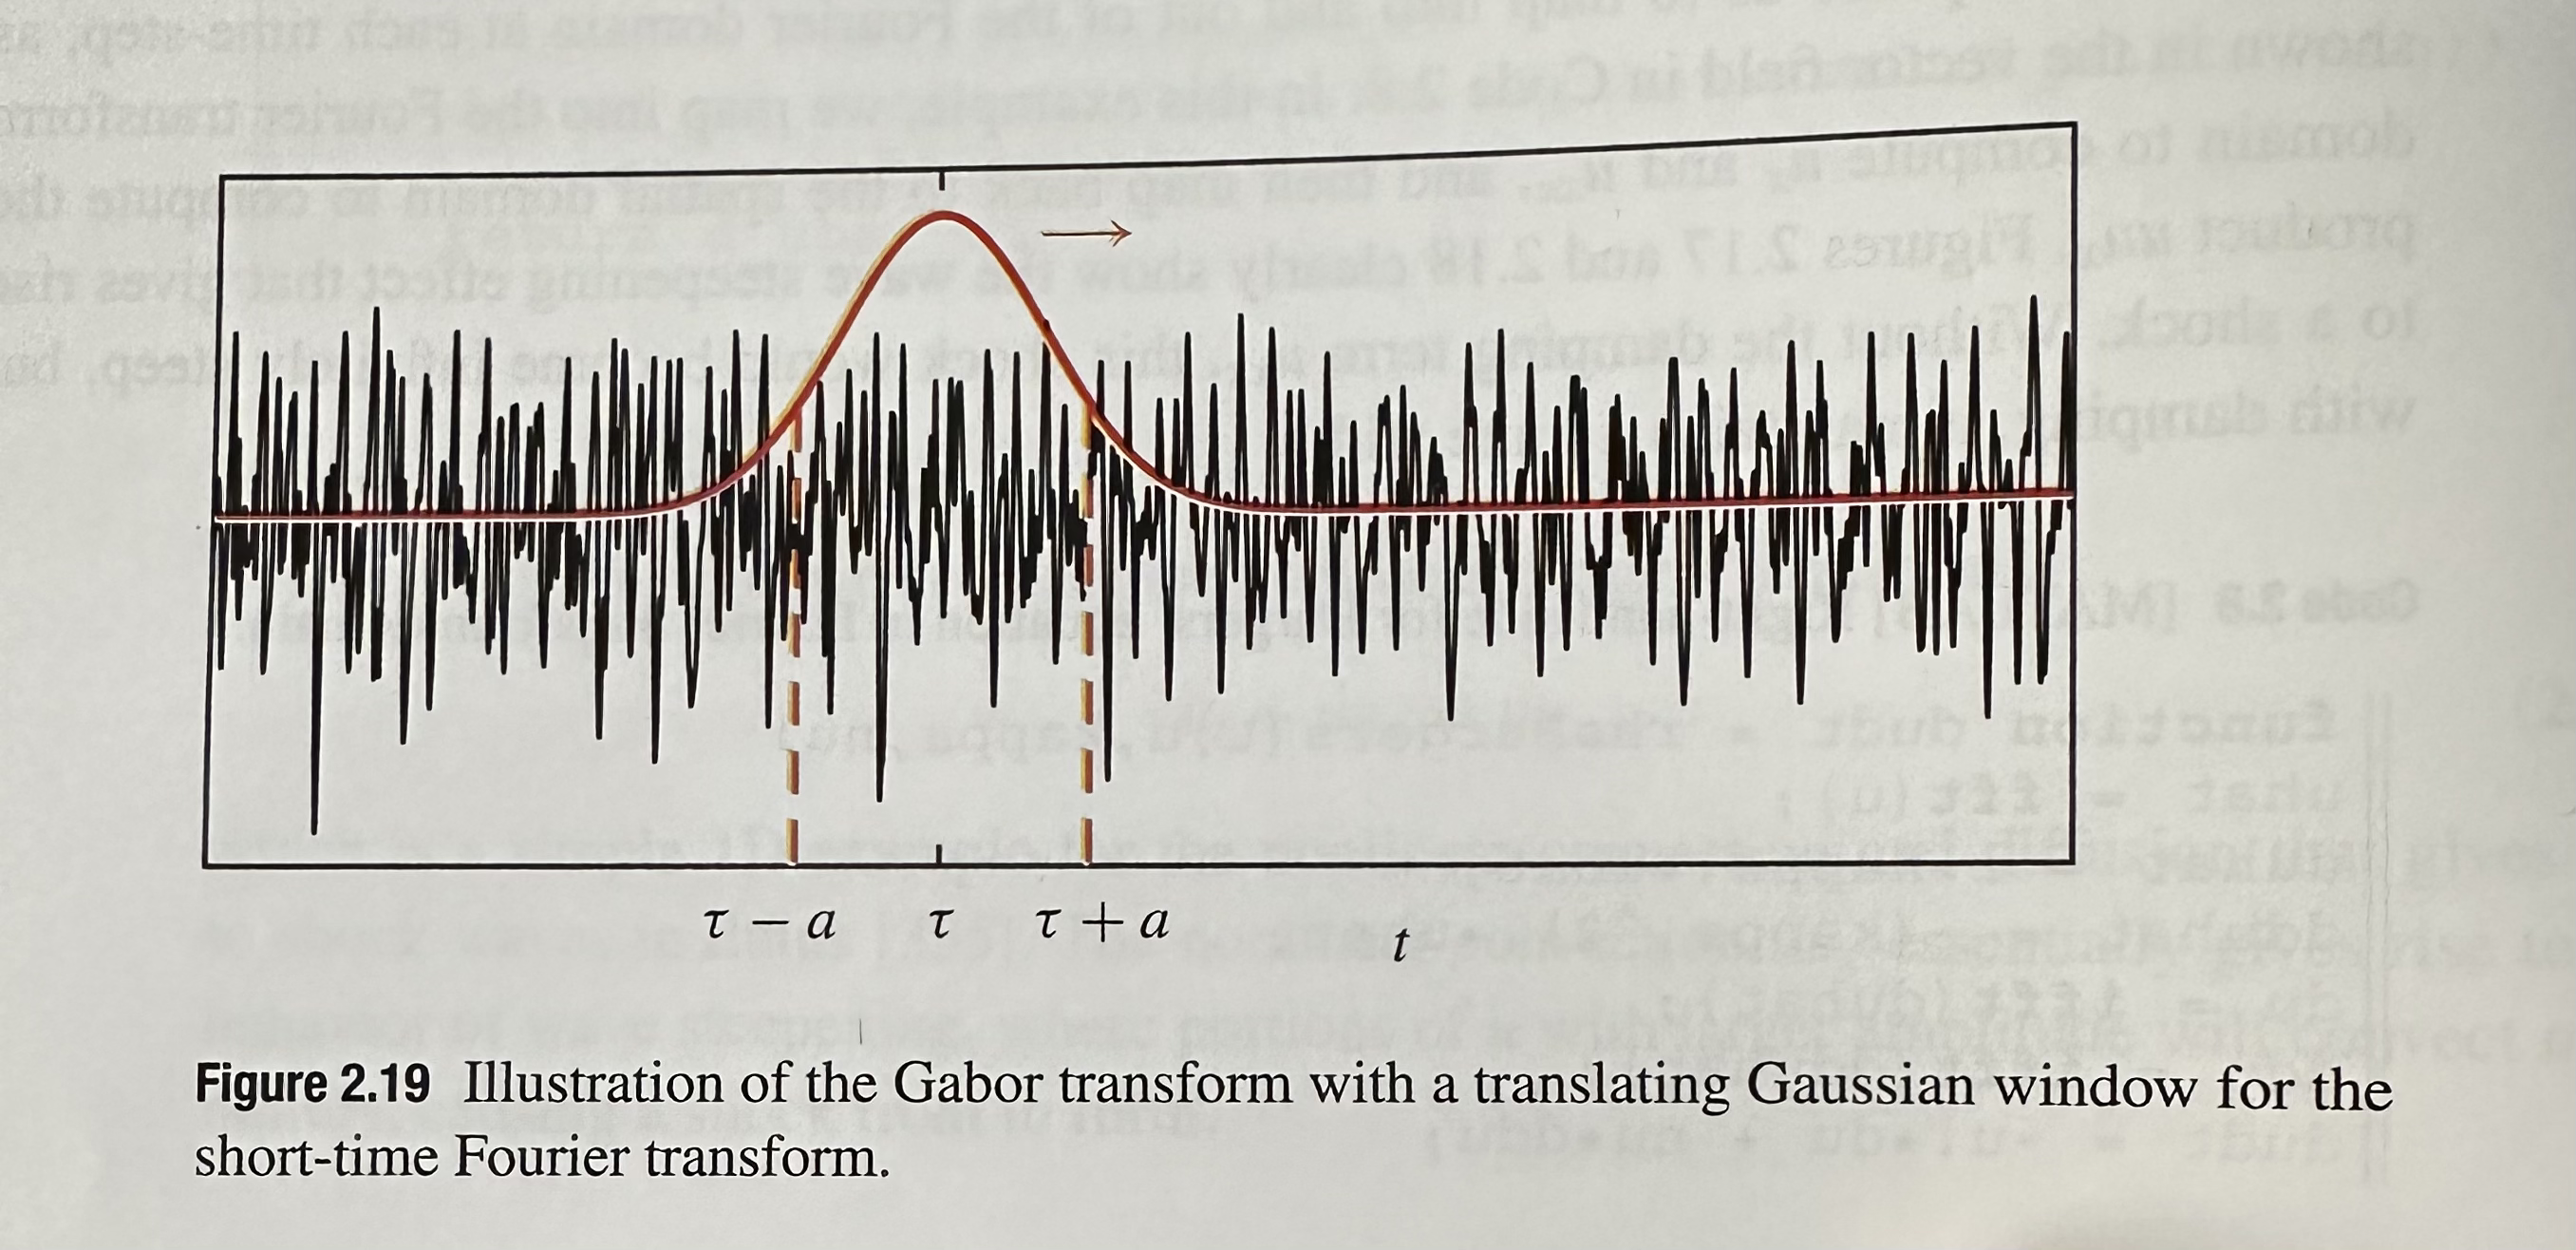
\includegraphics[width=0.7\linewidth]{Figures/Kernel_Example_STFT.png}
            \caption{Example of a Kernel Function for STFT}
            \label{fig:Kernel_Func_STFT}
        \end{figure}
    \end{itemize}
    \item The Inverse STFT is:
    \begin{equation*}
        f(t) = G^{-1}(\hat{f}_g(t,\omega)) = \frac{1}{2\pi \Vert g\Vert^2}\int_{-\infty}^{\infty}\int_{-\infty}^{\infty} \hat{f}_g(\tau, \omega)g(t-\tau)e^{i\omega t}d\omega dt
    \end{equation*}
    
\end{itemize}

\subsubsection*{Discrete Gabor Transform}

\begin{itemize}
    \item For the \textbf{Discrete Gabor Transform} one needs to discretize in both frequency and time.
    \begin{align*}
        v &= j\Delta\omega \\
        \tau &= k\Delta\tau
    \end{align*}
    \item The discretized kernel function is the following:
    \begin{equation*}
        g_{j,k} e^{i2\pi j\Delta\omega t}g(t-k\Delta t)
    \end{equation*}
    \item The discrete Gabor transform is the following:
    \begin{equation*}
        \hat{f}_{j, k} = \left<f,g_{j,k}\right> = \int_{-\infty}^{\infty} f(\tau)\bar{g}(\tau)d\tau
    \end{equation*}
    The integral can be solved numerically using Riemann sums.
\end{itemize}

\subsubsection*{Examples of using Gabor Transform}
% Will add to this when going through practice problems

\subsection*{Wavelets and Multi-Resolution Analysis}
\href{https://chatgpt.com/c/683210e2-ed70-800a-ab69-dfbfabae2915}{Some Additional information from Chat GPT on this section}
\begin{itemize}
    \item Wavelets extend the concept of Fourier Analysis by extending it to more general orthogonal bases. Furthermore, it partially overcomes the uncertainty principle by making use of \textbf{multi-resolution decomposition}.
    \begin{itemize}
        \item \textbf{From ChatGPT:} The \textbf{uncertainty principle} in the context of the Fourier transform is the trade-off in precision between the time (or spatial) and frequency domains. 
        \begin{itemize}
            \item Specifically, if a signal is localized to a specific period of time, the frequency content must be spread out.  
            \item On the other hand, if the signal is associated with a specific range of frequencies, it must be infinite in time.
        \end{itemize}
        \item \textbf{From ChatGPT:} The concept of \textbf{multi-resolution analysis} is a technique in signal processing where a signal is analyzed at multiple levels of resolution or scale, allowing one to analyze the signal's global structure and finer details.
        \begin{figure}[hbt!]
            \centering
            \includegraphics[width=0.4\linewidth]{Figures/Uncertainty_principle_Fourier_analysis.png}
            \caption{Representation of the uncertainty principle in the context of Fourier analysis}
            \label{fig:Uncertainty Principle FT}
        \end{figure}
        \item \textbf{From ChatGPT:} Why are orthogonal basis important:
        \begin{itemize}
            \item In linear algebra (in general) orthogonal basis are important for three reasons:
            \begin{enumerate}
                \item Simplified computations. Specifically, dot products, projections, and decompositions are easier
                \item Orthogonal matrices maintain their lengths and angles. Furthermore, symmetric matrices can be diagonalized using orthogonal eigenvectors (aka. Spectral Theorem).
                \item Numerical stability, as using orthogonal basis reduces errors due to rounding and floating point precision. This is because orthogonal bases are linearly independent. Therefore, linear dependencies can be avoided, which can amplify errors.
            \end{enumerate}
            \item In Fourier analysis, orthogonality matters for the following reasons:
            \begin{enumerate}
                \item allows for better signal decomposition (as the signal can be represented as a sum of orthogonal components).
                \item Invertibility and uniqueness
                \item compression and filtering
            \end{enumerate}
        \end{itemize}
    \end{itemize}
    \item Basic idea around how \textbf{Wavelet Analysis} work:
    \begin{enumerate}
        \item It starts with the \textbf{mother wavelet}. This function will then be used to generate a family of scaled and translated versions.
        \begin{equation*}
            \psi_{a, b}(t) = \frac{1}{\sqrt{a}}\psi\left( \frac{t-b}{a} \right)
        \end{equation*}
        Where $a$ and $b$ are factors used for scaling (high vs low frequency) and translating (changing in time), respectively.
        \item An example of a wavelet is the \textbf{Haar} wavelet:
        \begin{equation*}
            \psi(t) = \begin{cases}
                1 & \text{for } 0 \leq t < \frac{1}{2}, \\
                -1 & \text{for } \frac{1}{2} \leq t < 1, \\
                0 & \text{otherwise }
            \end{cases}
        \end{equation*}
        By choosing each higher frequency layer as a bisection of the lower layers, the \textbf{Haar} wavelets are orthogonal (thus they are a great basis for a signal).
        \item \textbf{Summary:} Wavelets are like \hl{mathematical microscopes} that are used to analyze signals at different scales. They can capture local transient features such as edges, spikes, or sudden changes. Methods like DWT (Discrete Wavelet Transform) and CWT (Continuous Wavelet Transform), albeit to a lesser extent, use the wavelets in conjunction with multi-resolution decomposition to reveal the time-frequency characteristics.
        \begin{itemize}
            \item \textit{Think of STFT as a fixed magnifying glass - you see everything with the same “zoom level,” which limits your ability to resolve very fast or very slow changes well.} 
            \item \textit{Wavelet Transform, on the other hand, is like a variable zoom magnifying glass -  you zoom in tightly on fast events (good time resolution) and zoom out to see slow trends clearly (good frequency resolution).}
        \end{itemize}
    \end{enumerate}
    \item Continuous Wavelet Transform (CWT):
    \begin{enumerate}
        \item 
    \end{enumerate}
\end{itemize}


\end{document}